\chapter{Induction}\label{induction_chap}
%\hyperdef{in}{duction}

\emph{Induction} is a powerful method for showing a property is true
for all nonnegative integers.  Induction plays a central role in
discrete mathematics and computer science.  In fact, its use is a
defining characteristic of \emph{discrete}---as opposed to
\emph{continuous}---mathematics.  This chapter introduces two
versions of induction, Ordinary and Strong, and explains why they work
and how to use them in proofs.  It also introduces the Invariant
Principle, which is a version of induction specially adapted for
reasoning about step-by-step processes.


\iffalse
we'll introduce induction and a variant called \term{strong
induction}.  Although these two version of methods look and feel
different, it turns out that they are equivalent in the sense that a
proof using any one of the methods can be automatically reformatted so
that it becomes a proof using any of the other methods.  The choice of
which method to use is up to you and typically depends on whichever
seems to be the easiest or most natural for the problem at hand.
\fi


\section{Ordinary Induction}\label{ordinary_induct_chap}
\label{ordinary_induct_sec}

To understand how induction works, suppose there is a professor who
brings a bottomless bag of assorted miniature candy bars to her large
class.  She offers to share the candy in the following way.  First,
she lines the students up in order.  Next she states two rules:

\begin{enumerate}
\item The student at the beginning of the line gets a candy bar.
\item If a student gets a candy bar, then the following student in line
  also gets a candy bar.
\end{enumerate}
%
Let's number the students by their order in line, starting the count with
0, as usual in computer science.  Now we can understand the second rule as
a short description of a whole sequence of statements:
%
\begin{itemize}
\item If student 0 gets a candy bar, then student 1 also gets one.
\item If student 1 gets a candy bar, then student 2 also gets one.
\item If student 2 gets a candy bar, then student 3 also gets one.

\hspace{1.2in} \vdots
\end{itemize}
%
Of course, this sequence has a more concise mathematical description:
\begin{quote}
  If student $n$ gets a candy bar, then student $n+1$ gets a
  candy bar, for all nonnegative integers $n$.
\end{quote}
So suppose you are student 17.  By these rules, are you entitled to a
miniature candy bar?  Well, student 0 gets a candy bar by the first
rule.  Therefore, by the second rule, student 1 also gets one, which
means student 2 gets one, which means student 3 gets one as well, and
so on.  By 17 applications of the professor's second rule, you get
your candy bar!  Of course the rules really guarantee a candy bar to
\emph{every} student, no matter how far back in line they may be.

\subsection{A Rule for Ordinary Induction}\label{ord_induction_subsec}

The reasoning that led us to conclude that every student gets a candy bar is 
essentially all there is to induction.
\textbox{ 
\textboxtitle{The Induction Principle.}
\index{induction|textbf}

Let $P$ be a predicate on nonnegative integers.  If
%
\noindent \begin{itemize}
\item $P(0)$ is true, and
\item $P(n) \QIMPLIES P(n+1)$ for all nonnegative integers, $n$,
\end{itemize}
then
\begin{itemize}
\item $P(m)$ is true for all nonnegative integers, $m$.
\end{itemize}
}
\iffalse
So our claim that all the Professor's students get a candy bar was simply
an application of the Induction Rule with $P(n)$ defined to be the
predicate, ``student $n$ gets a candy bar.''
\fi

Since we're going to consider several useful variants of induction in
later sections, we'll refer to the induction method described above as
\emph{ordinary induction} when we need to distinguish it.  Formulated
as a proof rule as in Section~\ref{logical_deductions_subsec}, this
would be
\begin{rul*} \inductioncase{Induction Rule}
\Rule{P(0), \quad \forall n \in \naturals.\, P(n) \QIMPLIES P(n+1)}
{\forall m \in \naturals.\, P(m)}
\end{rul*}

This Induction Rule works for the same intuitive reason that all
the students get candy bars, and we hope the explanation using candy bars
makes it clear why the soundness of ordinary induction can be taken
for granted.  In fact, the rule is so obvious that it's hard to see what
more basic principle could be used to justify it.\footnote{But see
Section~\ref{versusWO}.}  What's not so obvious is how much mileage 
we get by using it.

\subsection{A Familiar Example}

Below is the formula~\eqref{sum-to-n-again} for the sum of the
nonnegative integers up to $n$.  The formula holds for all nonnegative
integers, so it is the kind of statement to which induction applies
directly.  We've already proved this formula using the Well
  Ordering Principle (Theorem~\ref{sum_to_n_thm}), but now we'll
prove it \emph{by induction}, that is, using the Induction Principle.
\begin{theorem}\label{sum-to-n-again-theorem}
For all $n \in \naturals$,
\begin{equation}\label{sum-to-n-again}
1 + 2 + 3 + \cdots + n = \frac{n(n+1)}{2}
\end{equation}
\end{theorem}

To prove the theorem by induction, define predicate $P(n)$ to be the
equation~\eqref{sum-to-n-again}.  Now the theorem can be restated as
the claim that $P(n)$ is true for all $n \in \naturals$.  This is
great, because the Induction Principle lets us reach precisely that
conclusion, provided we establish two simpler facts:
\begin{itemize}
\item $P(0)$ is true.
\item For all $n \in \naturals$, $P(n) \QIMPLIES P(n+1)$.
\end{itemize}
So now our job is reduced to proving these two statements.

The first statement follows because of the convention that a sum of
zero terms is equal to 0.  So $P(0)$ is the true assertion that a sum
of zero terms is equal to $0(0+1)/2 = 0$.

The second statement is more complicated.  But remember the basic
plan from Section~\ref{sec:prove_implies} for proving the validity of
any implication: \emph{assume} the statement on the left and then
\emph{prove} the statement on the right.  In this case, we assume
$P(n)$---namely, equation~\eqref{sum-to-n-again}---in order to prove
$P(n+1)$, which is the equation
\begin{equation}\label{sum-to-n-again-Pn1}
1 + 2 + 3 + \cdots + n + (n+1) = \frac{(n+1)(n+2)}{2}.
\end{equation}
These two equations are quite similar; in fact, adding $(n+1)$ to both
sides of equation~\eqref{sum-to-n-again} and simplifying the right side 
gives the equation~\eqref{sum-to-n-again-Pn1}:
\begin{align*}
1 + 2 + 3 + \cdots + n + (n+1)
    & = \frac{n(n+1)}{2} + (n+1) \\
    & = \frac{(n+2)(n+1)}{2}
\end{align*}
Thus, if $P(n)$ is true, then so is $P(n+1)$.  This argument is valid
for every nonnegative integer $n$, so this establishes the second fact
required by the induction proof.  Therefore, the Induction Principle
says that the predicate $P(m)$ is true for all nonnegative integers,
$m$.  The theorem is proved.

\iffalse
In effect, we've just proved
that $P(0)$ implies $P(1)$, $P(1)$ implies $P(2)$, $P(2)$ implies
$P(3),\dots$, all in one fell swoop.
\fi

\subsection{A Template for Induction Proofs}
\label{templ-induct-proofs}

The proof of equation~\eqref{sum-to-n-again} was relatively simple,
but even the most complicated induction proof follows exactly the same
template.  There are five components:

\begin{enumerate}

\item \textbf{State that the proof uses induction.}  This immediately
  conveys the overall structure of the proof, which helps your reader
  follow your argument.

\item \textbf{Define an appropriate predicate $P(n)$.}  The predicate
  $P(n)$ is called the 
\emph{induction hypothesis}\index{induction!induciton hypothesis}.  The eventual
  conclusion of the induction argument will be that $P(n)$ is true for
  all nonnegative $n$.  A clearly stated induction hypothesis is often
  the most important part of an induction proof, and its omission is
  the largest source of confused proofs by students.

In the simplest cases, the induction hypothesis can be lifted straight
from the proposition you are trying to prove, as we did with
equation~\eqref{sum-to-n-again}.  Sometimes the induction hypothesis
will involve several variables, in which case you should indicate
which variable serves as $n$.

\item \textbf{Prove that $P(0)$ is true.}  This is usually easy, as in the
  example above.  This part of the proof is called the \emph{base case}%
\index{base case|see{induction}}
  or \emph{basis step}.\iffalse
  (Sometimes the base case will be $n=1$ or even
  some larger number, in which case the starting value of $n$ also should
  be stated.)\fi

\item \textbf{Prove that $P(n)$ implies $P(n+1)$ for every nonnegative
  integer $n$.}  This is called the \emph{inductive
  step}\index{induction!inductive step}.  The basic plan is always the
  same: assume that $P(n)$ is true and then use this assumption to
  prove that $P(n+1)$ is true.  These two statements should be fairly
  similar, but bridging the gap may require some ingenuity.  Whatever
  argument you give must be valid for every nonnegative integer $n$,
  since the goal is to prove that \emph{all} the following
  implications are true:
\[
P(0) \rightarrow P(1),\  P(1) \rightarrow  P(2),\  P(2) \rightarrow P(3), \dots.
\]

\item \textbf{Invoke induction.}  Given these facts, the induction
  principle allows you to conclude that $P(n)$ is true for all nonnegative
  $n$.  This is the logical capstone to the whole argument, but it is so
  standard that it's usual not to mention it explicitly.

\end{enumerate}

Always be sure to explicitly label the \emph{base case} and the
\emph{inductive step}.  Doing so will make your proofs clearer and
will decrease the chance that you forget a key step---like checking
the base case.

\subsection{A Clean Writeup}

The proof of Theorem~\ref{sum-to-n-again-theorem} given above is
perfectly valid; however, it contains a lot of extraneous explanation
that you won't usually see in induction proofs.  The writeup below is
closer to what you might see in print and should be prepared to
produce yourself.

\begin{proof}[Revised proof of Theorem~\ref{sum-to-n-again-theorem}]
We use induction.  The induction hypothesis, $P(n)$, will be
equation~\eqref{sum-to-n-again}.

\inductioncase{Base case}: $P(0)$ is true, because both sides of
equation~\eqref{sum-to-n-again} equal zero when $n=0$.

\inductioncase{Inductive step}: Assume that $P(n)$ is true, that is
equation~\eqref{sum-to-n-again} holds for some nonnegative integer
$n$.  Then adding $n+1$ to both sides of the equation implies that
\begin{align*}
1 + 2 + 3 + \cdots + n + (n+1)
    & = \frac{n(n+1)}{2} + (n+1)\\\iffalse  & \text{(by induction hypothesis)} \fi
    & = \frac{(n+1)(n+2)}{2}  & \text{(by simple algebra)}
\end{align*}
which proves $P(n+1)$.

So it follows by induction that $P(n)$ is true for all nonnegative $n$.
\end{proof}

It probably bothers you that induction led to a proof of this
summation formula but did not provide an intuitive way to understand
it nor did it explain where the formula came from in the first
place.\footnote{Methods for finding such formulas are covered in
  Part~III of the text.}  This is both a weakness and a strength.  It
is a weakness when a proof does not provide insight.  But it is a
strength that a proof can provide a reader with a reliable guarantee
of correctness without \emph{requiring} insight.

\iffalse
\subsection{Powers of Odd Numbers}

\begin{fact*}
The $n$th power of an odd number is odd, for all nonnegative integers, $n$.
\end{fact*}
The proof in Chapter~\ref{C01} that $\sqrt[n]{2}$ is irrational used this 
``obvious'' fact.  Instead of taking it for granted, we can prove this fact
by induction.
The proof will require a simple Lemma.
\begin{lemma*}
The product of two odd numbers is odd.
\end{lemma*}
To prove the Lemma, note that the odd numbers are, by definition, the
numbers of the form $2k+1$ where $k$ is an integer.  But
\[
(2k+1)(2k'+1) = 2(2kk' + k + k')+1,
\]
so the product of two odd numbers also has the form of an odd number,
which proves the Lemma.

Now we will prove the Fact using the induction hypothesis
\[
P(n) \eqdef \text{if $a$ is an odd integer, then so is $a^{n}$}.
\]

The base case $P(0)$ holds because $a^{0} =1$, and 1 is odd.

For the inductive step, suppose $n\geq 0$, $a$ is an odd number and $P(n)$
holds.  So $a^n$ is an odd number.  Therefore, $a^{n+1} = a^{n}a$ is a
product of odd numbers, and by the Lemma $a^{n+1}$ is also odd.  This
proves $P(n+1)$, and we conclude by induction that $P(n)$ holds for
nonnegative integers $n$.
\fi

\iffalse
An alternative proof of Lemma~\ref{finmin} that every partial order on a
nonempty finite set has a minimal element can be based on induction.  This
time there is no $n$ mentioned, so we better find one.

We'll use the induction hypothesis
\[
P(n) \eqdef \text{a strict partial order on a set of size $n$ has a minimal
  element}.
\]

As a base case, we'll use $n=1$.  Now $P(1)$ holds because in a
one-element partial order, the element is minimal (and maximal) by
definition.

For the inductive step, assume $P(n)$ holds and consider a strict partial
order, $R$, on a set, $A$, of size $n+1$ for $n \geq 1$.  We will prove
that $A$ has a minimal element.

Now $A$ has 2 or more elements, so pick one and call it $a_0$.  If $a_0$
is a minimal element, then we are done.  Otherwise, let $A'$ be the set $A
- \set{a_0}$ and $R'$ be the relation $R$ restricted to $A'$.

Now it's easy to check that $R'$ is a strict partial order on set $A'$
whose size is $n$.  So by induction, there is an $R'$-minimal element, $m
\in A'$.  We claim that $m$ is also a minimal element of $A$.

Now there is no element $a' \in A'$ such that $a'\,R\,m$, so to prove
$m$ is minimal in $A$,  as long as it is not true that $a_0\,R\, m$

This element $m$ will also be minimal in $A$ unless

Since $a_0$ is not minimal, there is an element $a_1 \in A'$ such that
$a_1\,R\,a_0$.

\fi

\subsection{A More Challenging Example}\label{subsec:tile_induction}

During the development of MIT's famous Stata Center, as costs rose
further and further beyond budget, some radical fundraising ideas were
proposed.  One rumored plan was to install a big square courtyard
divided into unit squares.  The big square would be $2^n$ units on a
side for some undetermined nonnegative integer $n$, and one of the
unit squares in the center\footnote{In the special case $n = 0$, the
  whole courtyard consists of a single central square; otherwise,
  there are four central squares.} occupied by a statue of a wealthy
potential donor---whom the fund raisers privately referred to as
``Bill.''  The $n = 3$ case is shown in Figure~\ref{fig:2nx2n-tile}.

\begin{figure}

\graphic{Fig_3-1}

\caption{A $2^n \times 2^n$ courtyard for $n = 3$.}
\label{fig:2nx2n-tile}
\end{figure}

A complication was that the building's unconventional architect, Frank
Gehry, was alleged to require that only special L-shaped tiles (shown
in Figure~\ref{fig:Ltile}) be used for the courtyard.  For $n = 2$, a
courtyard meeting these constraints is shown in
Figure~\ref{fig:2Ltile}.  But what about for larger values of~$n$?  Is
there a way to tile a $2^n \times 2^n$ courtyard with L-shaped tiles
around a statue in the center?  Let's try to prove that this is so.

\begin{figure}

\graphic{Fig_3-2}

\caption{The special L-shaped tile.}
\label{fig:Ltile}
\end{figure}

\begin{figure}

\graphic{Fig_3-3}

\caption{A tiling using L-shaped tiles for $n = 2$ with Bill in a
  center square.}
\label{fig:2Ltile}
\end{figure}

\begin{theorem}\label{bill}
For all $n \geq 0$ there exists a tiling of a $2^n \times 2^n$
courtyard with Bill in a central square.
\end{theorem}

\begin{proof}
\emph{(doomed attempt)} The proof is by induction.  Let $P(n)$ be the
proposition that there exists a tiling of a $2^n \times 2^n$ courtyard
with Bill in the center.

\inductioncase{Base case}: $P(0)$ is true because Bill fills the whole courtyard.

\inductioncase{Inductive step}: Assume that there is a tiling of a
$2^n \times 2^n$ courtyard with Bill in the center for some $n \geq
0$.  We must prove that there is a way to tile a $2^{n+1} \times
2^{n+1}$ courtyard with Bill in the center \dots.
\end{proof}

Now we're in trouble!  The ability to tile a smaller courtyard with Bill
in the center isn't much help in tiling a larger courtyard with Bill in
the center.  We haven't figured out how to bridge the gap between $P(n)$
and $P(n+1)$.

So if we're going to prove Theorem~\ref{bill} by induction, we're going to
need some \emph{other} induction hypothesis than simply the statement
about $n$ that we're trying to prove.


\iffalse
\textbf{Maybe you can figure out a good induction hypothesis for
  tiling.  In class we'll present some hypotheses that do work.}
\fi

%\iffalse  %Unhide after lecture:

When this happens, your first fallback should be to look for a
\emph{stronger} induction hypothesis; that is, one which implies
your previous hypothesis.  For example, we could make $P(n)$ the
proposition that for \emph{every} location of Bill in a $2^n \times
2^n$ courtyard, there exists a tiling of the remainder.

This advice may sound bizarre: ``If you can't prove something, try to
prove something grander!''  But for induction arguments, this makes
sense.  In the inductive step, where you have to prove $P(n) \QIMPLIES
P(n+1)$, you're in better shape because you can \emph{assume} $P(n)$,
which is now a more powerful statement.  Let's see how this plays out
in the case of courtyard tiling.

\begin{proof}[Proof (successful attempt)]
The proof is by induction.  Let $P(n)$ be the proposition that for
every location of Bill in a $2^n \times 2^n$ courtyard, there exists a
tiling of the remainder.

\inductioncase{Base case}: $P(0)$ is true because Bill fills the
whole courtyard.

\inductioncase{Inductive step}: Assume that $P(n)$ is true for some
$n \geq 0$; that is, for every location of Bill in a $2^n \times 2^n$
courtyard, there exists a tiling of the remainder.  Divide the
$2^{n+1} \times 2^{n+1}$ courtyard into four quadrants, each $2^n
\times 2^n$.  One quadrant contains Bill (\textbf{B} in the diagram
below).  Place a temporary Bill (\textbf{X} in the diagram) in each of
the three central squares lying outside this quadrant as shown in
Figure~\ref{fig:stronger-bill}.

\begin{figure}

\graphic{Fig_3-4}

\caption{Using a stronger inductive hypothesis to prove
  Theorem~\ref{bill}.}
\label{fig:stronger-bill}
\end{figure}

Now we can tile each of the four quadrants by the induction
assumption.  Replacing the three temporary Bills with a single
L-shaped tile completes the job.  This proves that $P(n)$ implies
$P(n+1)$ for all $n \geq 0$.  Thus $P(m)$ is true for all $m \in
\naturals$, and the theorem follows as a special case where we put
Bill in a central square.
\end{proof}

This proof has two nice properties.  First, not only does the argument
guarantee that a tiling exists, but also it gives an algorithm for
finding such a tiling.  Second, we have a stronger result: if Bill
wanted a statue on the edge of the courtyard, away from the pigeons,
we could accommodate him!

Strengthening the induction hypothesis is often a good move when an
induction proof won't go through.  But keep in mind that the stronger
assertion must actually be \emph{true}; otherwise, there isn't much
hope of constructing a valid proof.  Sometimes finding just the right
induction hypothesis requires trial, error, and insight.  For example,
mathematicians spent almost twenty years trying to prove or disprove
the conjecture that every planar graph is
5-choosable.\footnote{5-choosability is a slight generalization
  of 5-colorability.  Although every planar graph is 4-colorable and
  therefore 5-colorable, not every planar graph is 4-choosable.  If
  this all sounds like nonsense, don't panic.  We'll discuss graphs,
  planarity, and coloring in Part~\ref{part:structures} of the text.}
Then, in 1994, Carsten Thomassen gave an induction proof simple enough
to explain on a napkin.  The key turned out to be finding an extremely
clever induction hypothesis; with that in hand, completing the
argument was easy!

%\fi  %end UnHide after lecture

\subsection{A Faulty Induction Proof}

If we have done a good job in writing this text, right about now you
should be thinking, ``Hey, this induction stuff isn't so hard after
all---just show $P(0)$ is true and that $P(n)$ implies $P(n+1)$ for
any number~$n$.''  And, you would be right, although sometimes when
you start doing induction proofs on your own, you can run into
trouble.  For example, we will now use induction to ``prove'' that all
horses are the same color---just when you thought it was safe to skip
class and work on your robot program instead.  Sorry!

\begin{falsethm*}
All horses are the same color.
\end{falsethm*}

Notice that no $n$ is mentioned in this assertion, so we're going to have
to reformulate it in a way that makes an $n$ explicit.  In particular,
we'll (falsely) prove that

\begin{falsethm}\label{horses}
In every set of $n \geq 1$ horses, all the horses are the same color.
\end{falsethm}

This is a statement about all integers $n \geq 1$ rather $\geq 0$, so it's
natural to use a slight variation on induction: prove $P(1)$ in the base
case and then prove that $P(n)$ implies $P(n+1)$ for all $n \geq 1$ in the
inductive step.  This is a perfectly valid variant of induction and is
\emph{not} the problem with the proof below.

\begin{bogusproof}

The proof is by induction on $n$.  The induction hypothesis, $P(n)$,
will be
\begin{equation}\label{horsehyp}
\text{In every set of $n$ horses, all are the same color.}
\end{equation}

\inductioncase{Base case}: ($n=1$).  $P(1)$ is true, because in a
size-1 set of horses, there's only one horse, and this horse is
definitely the same color as itself.

\inductioncase{Inductive step}: Assume that $P(n)$ is true for some $n \geq 1$.
That is, assume that in every set of $n$ horses, all are the same color.
Now suppose we have a set of $n+1$ horses:
\[
h_1,\ h_2,\ \dots,\ h_n,\ h_{n+1}.
\]
We need to prove these $n+1$ horses are all the same color.

By our assumption, the first $n$ horses are the same color:
\[
\underbrace{h_1,\ h_2,\ \dots,\ h_n}_{\text{same color}}, h_{n+1}
\]
Also by our assumption, the last $n$ horses are the same color:
\[
h_1,\ \underbrace{h_2,\ \dots,\ h_n,\ h_{n+1}}_{\text{same color}}
\]
So $h_1$ is the same color as the remaining horses besides $h_{n+1}$
---that is, $h_2, \dots, h_n$.  Likewise, $h_{n+1}$ is the same
color as the remaining horses besides $h_1$---that is, $h_2, \dots,
h_n$, again.  Since $h_1$ and $h_{n+1}$ are the same color as $h_2,
\dots, h_n$, all $n+1$ horses must be the same color, and so $P(n+1)$
is true.  Thus, $P(n)$ implies $P(n+1)$.

By the principle of induction, $P(n)$ is true for all $n \geq 1$.
\end{bogusproof}
We've proved something false!  Does this mean that math broken and we
should all take up poetry instead?  Of course not!  It just means
that this proof has a mistake.

%hide after lecture:
\iffalse

\textbf{See if you can figure it out before we take it up in class.}
\fi

%end hide

%\iffalse %UNHIDE after lecture

The mistake in this argument is in the sentence that begins ``So $h_1$
is the same color as the remaining horses besides $h_{n+1}$---that is
$h_2, \dots, h_n, \dots$.''  The ellipis notation (``$\dots$'') in the
expression ``$h_1, h_2, \dots, h_n, h_{n+1}$'' creates the impression
that there are some remaining horses---namely $h_2, \dots, h_n$
---besides $h_1$ and $h_{n+1}$.  However, this is not true when $n =
1$.  In that case, $h_1, h_2, \dots, h_n, h_{n+1}$ is just $h_1, h_2$
and \emph{there are no ``remaining'' horses} for $h_1$ to share a
color with.  And of course, in this case $h_1$ and $h_2$ really don't
need to be the same color.

This mistake knocks a critical link out of our induction argument.  We
proved $P(1)$ and we \emph{correctly} proved $P(2) \implies P(3)$, $P(3)
\implies P(4)$, etc.  But we failed to prove $P(1) \implies P(2)$, and so
everything falls apart: we cannot conclude that $P(2)$, $P(3)$, etc., are
true.  And naturally, these propositions are all false; there are
sets of $n$ horses of different colors for all $n \ge 2$.

%\fi

%end unhide

Students sometimes explain that the mistake in the proof is because
$P(n)$ is false for $n \geq 2$, and the proof assumes something false,
$P(n)$, in order to prove $P(n+1)$.  You should think about how to
help such a student understand why this explanation would get no
credit on a Math for Computer Science exam.

%% Ordinary Induction Problems %%%%%%%%%%%%%%%%%%%%%%%%%%%%%%%%%%%%%%%%%%%%%%%%
\begin{problems}

\practiceproblems
\pinput{TP_min_of_finite_induction}
\pinput{TP_a_bogus_tiling_induction}

\classproblems
\pinput{CP_cubic_series}
\pinput{CP_geometric_series_induction}
\pinput{CP_sum_of_inverse_squares_induction}
\pinput{CP_courtyard_tiling_corner}
%\pinput{CP_flawed_induction_proof}
\pinput{CP_bogus_arithmetic_series_proof}

\homeworkproblems
\pinput{PS_fib_induction}
\pinput{PS_ripple_carry_adder_correctness}
\pinput{PS_periphery_length_game}
\pinput{PS_distributive-law-for-sets-by-induction}
\pinput{PS_koch_induction}

\examproblems
\pinput{MQ_sum_of_cubes}
\pinput{FP_induction_plus_2} 
\pinput{FP_sat_count_induction}
\pinput{FP_m_envelopes_induction}


\end{problems}

\section{Strong Induction}\label{strong_ind_sec}

A useful variant of induction is called \term{strong induction}.  Strong
induction and ordinary induction are used for exactly the same thing:
proving that a predicate is true for all nonnegative integers.  Strong
induction is useful when a simple proof that the predicate holds for $n+1$
does not follow just from the fact that it holds at $n$, but from the fact
that it holds for other values $ \le n$.

\subsection{A Rule for Strong Induction}

\textbox{
\textboxtitle{Principle of Strong Induction.}

Let $P$ be a predicate on  nonnegative integers.  If
\begin{itemize}
\item $P(0)$ is true, and
\item for all $n \in \naturals$, $P(0)$, $P(1)$, \dots, $P(n)$
\emph{together} imply $P(n+1)$,
\end{itemize}
then $P(m)$ is true for all $m \in \naturals$.
}

The only change from the ordinary induction principle is that strong
induction allows you make more assumptions in the inductive step of
your proof!  In an ordinary induction argument, you assume that $P(n)$
is true and try to prove that $P(n+1)$ is also true.  In a strong
induction argument, you may assume that $P(0)$, $P(1)$, \dots, and
$P(n)$ are \emph{all} true when you go to prove $P(n+1)$.  So you can
assume a \emph{stronger} set of hypotheses which can make your job
easier.

Formulated as a proof rule, strong induction is
\begin{rul*} \textbf{Strong Induction Rule}
\Rule{P(0), \quad \forall n \in \naturals. \;
    \bigl(P(0) \QAND P(1) \QAND \dots \QAND P(n) \bigr) \QIMPLIES P(n+1)}
{\forall m \in \naturals.\, P(m)}
\end{rul*}

Stated more succintly, the rule is
\begin{rul*}% \textbf{Strong Induction Rule}
\Rule{P(0), \quad [\forall k \le n \in \naturals.\, P(k)] \QIMPLIES P(n+1)}
{\forall m \in \naturals.\, P(m)}
\end{rul*}

The template for strong induction proofs is identical to the template
given in Section~\ref{templ-induct-proofs} for ordinary induction
except for two things:
\begin{itemize}

\item
you should state that your proof is by strong induction, and

\item
you can assume that $P(0)$, $P(1)$, \dots, $P(n)$ are all true instead
of only $P(n)$ during the inductive step.

\end{itemize}

\subsection{Products of Primes}

As a first example, we'll use strong induction to re-prove
Theorem~\ref{factor_into_primes} which we previously proved using Well
Ordering.

\begin{theorem*}%\label{primprod}
Every integer greater than 1 is a product of primes.
\end{theorem*}

\begin{proof}
We will prove the Theorem by strong induction, letting the induction 
hypothesis, $P(n)$, be
\[
n \text{ is a product of primes}.
\]
So the Theorem will follow if we prove that $P(n)$ holds for all $n
\geq 2$.

\inductioncase{Base Case}: ($n=2$): $P(2)$ is true because $2$ is prime, so it is
a length one product of primes by convention.

\inductioncase{Inductive step}: Suppose that $n \geq 2$ and that every
number from 2 to $n$ is a product of primes.  We must show that
$P(n+1)$ holds, namely, that $n+1$ is also a product of primes.  We
argue by cases:

If $n+1$ is itself prime, then it is a length one product of primes by
convention, and so $P(n+1)$ holds in this case.

Otherwise, $n + 1$ is not prime, which by definition means $n+1 =
k\cdot m$ for some integers $k,m$ between 2 and $n$.  Now by the
strong induction hypothesis, we know that both $k$ and $m$ are
products of primes.  By multiplying these products, it follows
immediately that $k\cdot m = n+1$ is also a product of primes.
Therefore, $P(n+1)$ holds in this case as well.

So $P(n+1)$ holds in any case, which completes the proof by strong
induction that $P(n)$ holds for all ~$n \ge 2$.

\end{proof}

\subsection{Making Change}

The country Inductia, whose unit of currency is the Strong, has coins
worth 3\sg\ (3 Strongs) and 5\sg.  Although the Inductians have some
trouble making small change like 4\sg\ or 7\sg, it turns out that they
can collect coins to make change for any number that is at least 8
Strongs.

\begin{figure}

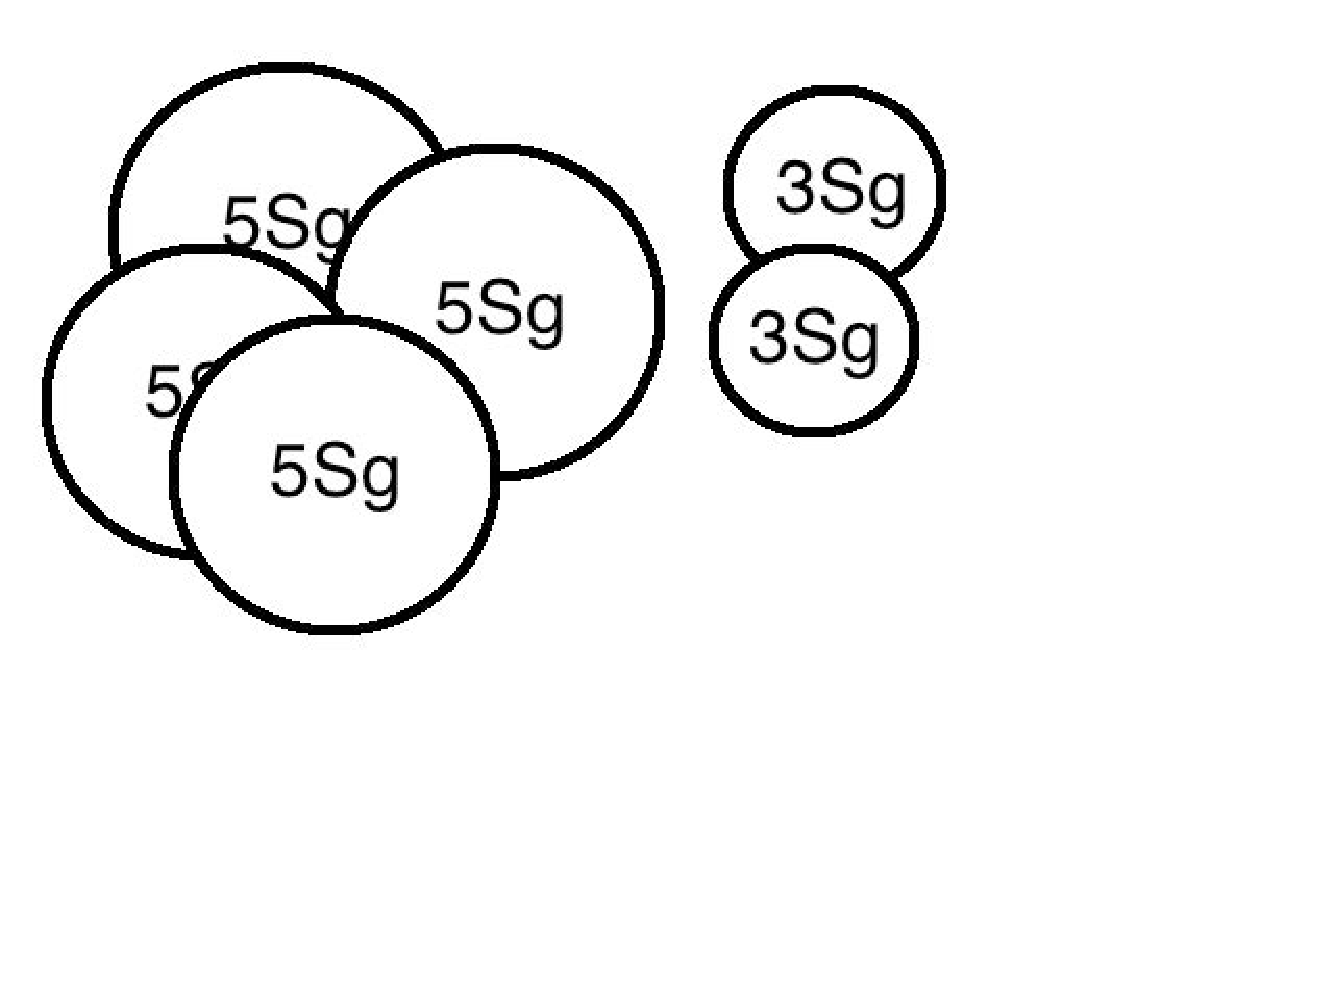
\includegraphics[trim = 0in 2.4in 2.5in 0in, clip, width = 3in]{Strong_Coins_image}
\caption{One way to make 26 Sg using Strongian currency}
\label{strong_coins}
\end{figure}

Strong induction makes this easy to prove for $n+1 \ge 11$, because then
$(n+1)-3 \ge 8$, so by strong induction the Inductians can make change for
exactly $(n+1)-3$ Strongs, and then they can add a 3\sg\ coin to get
$(n+1)\sg$.  So the only thing to do is check that they can make change
for all the amounts from 8 to 10\sg, which is not too hard to do.

Here's a detailed writeup using the official format:

\begin{proof}

  We prove by strong induction that the Inductians can make change for any
  amount of at least 8\sg.  The induction hypothesis, $P(n)$ will be:
\begin{quote}
There is a collection of coins whose value is $n+8$ Strongs.
\end{quote}

We now proceed with the induction proof:

\inductioncase{Base case}: $P(0)$ is true because a 3\sg\ coin together with
a 5\sg\ coin makes 8\sg.

\inductioncase{Inductive step}:  We assume $P(k)$ holds for all $k \leq n$, and
prove that $P(n+1)$ holds.  We argue by cases:

\textbf{Case} ($n+1$ = 1): We have to make $(n+1) +8 =9$\sg.  We can do this using three 3\sg\ coins.

\textbf{Case} ($n+1$ = 2): We have to make $(n+1) +8 =10$\sg.  Use two
5\sg\ coins.

\textbf{Case} ($n+1 \geq 3$): Then $0 \leq n - 2 \leq n$, so by the
strong induction hypothesis, the Inductians can make change for
$(n-2)+8$\sg.  Now by adding a 3\sg\ coin, they can make change for
$(n+1)+8\sg$, so $P(n+1)$ holds in this case.

Since $n \ge 0$, we know that $n + 1 \ge 1$ and thus that the three
cases cover every possibility.  Since $P(n+1)$ is true in every case,
we can conclude by strong induction that for all $n \ge 0$, the
Inductians can make change for $n+8$ Strong.  That is, they can make
change for any number of eight or more Strong.
\end{proof}

\subsection{The Stacking Game}\label{block-stack-subsection}

Here is another exciting game that's surely about to sweep the
nation!

%\hyperdef{stack}{game}
You begin with a stack of $n$ boxes.  Then you
make a sequence of moves.  In each move, you divide one stack of boxes
into two nonempty stacks.  The game ends when you have $n$ stacks, each
containing a single box.  You earn points for each move; in particular, if
you divide one stack of height $a + b$ into two stacks with heights $a$
and $b$, then you score $ab$ points for that move.  Your overall score is
the sum of the points that you earn for each move.  What strategy should
you use to maximize your total score?

As an example, suppose that we begin with a stack of $n = 10$ boxes.
Then the game might proceed as shown in Figure~\ref{fig:stacking-10}.
Can you find a better strategy?
%
\begin{figure}\redrawntrue
\[
\begin{array}{cccccccccccl}
\multicolumn{10}{c}{\textbf{Stack Heights}} & \quad & \textbf{Score} \\
\underline{10}&&&&&&&&& && \\
5&\underline{5}&&&&&&&& && 25 \text{ points} \\
\underline{5}&3&2&&&&&&& && 6 \\
\underline{4}&3&2&1&&&&&& && 4 \\
2&\underline{3}&2&1&2&&&&& && 4 \\
\underline{2}&2&2&1&2&1&&&& && 2 \\
1&\underline{2}&2&1&2&1&1&&& && 1 \\
1&1&\underline{2}&1&2&1&1&1&& && 1 \\
1&1&1&1&\underline{2}&1&1&1&1& && 1 \\
1&1&1&1&1&1&1&1&1&1 && 1 \\ \hline
\multicolumn{10}{r}{\textbf{Total Score}} & = & 45 \text{ points}
\end{array}
\]
\caption{An example of the stacking game with $n = 10$ boxes.  On each
line, the underlined stack is divided in the next step.}
\label{fig:stacking-10}
\end{figure}

\subsubsection{Analyzing the Game}

%Hide in full version
\iffalse
You will see in class how to use strong induction to analyze this game of
blocks.
\fi

%end Hide

%\iffalse  %unHide after Friday lecture:

Let's use strong induction to analyze the unstacking game.  We'll prove
that your score is determined entirely by the number of boxes---your
strategy is irrelevant!

\begin{theorem}\label{stacking}
Every way of unstacking $n$ blocks gives a score of $n(n-1)/2$ points.
\end{theorem}

There are a couple technical points to notice in the proof:

\begin{itemize}

\item The template for a strong induction proof mirrors the one for
  ordinary induction.

\item As with ordinary induction, we have some freedom to adjust indices.
In this case, we prove $P(1)$ in the base case and prove that $P(1),
\dots, P(n)$ imply $P(n+1)$ for all $n \geq 1$ in the inductive step.

\end{itemize}

\begin{proof}
The proof is by strong induction.  Let $P(n)$ be the proposition that
every way of unstacking $n$ blocks gives a score of $n(n-1)/2$.

\inductioncase{Base case}: If $n = 1$, then there is only one
block.  No moves are possible, and so the total score for the game is
$1(1 - 1)/2 = 0$.  Therefore, $P(1)$ is true.

\inductioncase{Inductive step}: Now we must show that $P(1)$, \dots, $P(n)$ imply
$P(n+1)$ for all $n \geq 1$.  So assume that $P(1)$, \dots, $P(n)$ are all
true and that we have a stack of $n+1$ blocks.  The first move must split
this stack into substacks with positive sizes $a$ and $b$ where $a+b =
n+1$ and $0<a,b\leq n$.  Now the total score for the game is the sum of
points for this first move plus points obtained by unstacking the two
resulting substacks:
%
\begin{align*}
\text{total score}
    & = \text{(score for 1st move)} \\
    & \quad + \text{(score for unstacking $a$ blocks)} \\
    & \quad + \text{(score for unstacking $b$ blocks)} \\
    & = ab + \frac{a(a-1)}{2} + \frac{b(b-1)}{2} & \text{by $P(a)$ and $P(b)$}\\
    & = \frac{(a+b)^2-(a+b)}{2} = \frac{(a+b)((a+b)-1)}{2}\\
    & = \frac{(n+1)n}{2}
\end{align*}
%
This shows that $P(1)$, $P(2)$, \dots, $P(n)$ imply $P(n+1)$.

Therefore, the claim is true by strong induction.
\end{proof}

%\fi
%end unHide

%% Strong Induction Problems %%%%%%%%%%%%%%%%%%%%%%%%%%%%%%%%%%%%%%%%%%%%%%%%%%

\begin{problems}
\practiceproblems
\pinput{TP_Induction_Rules}
\pinput{TP_a_bogus_fibonacci_induction}
\pinput{TP_another_bogus_fibonacci_induction}
\pinput{TP_Induction_by_n+3}

\classproblems
\pinput{CP_fibonacci_by_induction}
\pinput{CP_bogus_unique_prime_factors}
\pinput{CP_box_unstacking} %not strong induction, but depends on stacking game

\homeworkproblems
\pinput{PS_team_division}
\pinput{PS_bogus_prime_divides_integer_product}

\examproblems
\pinput{MQ_fib_squares}
\pinput{FP_3_exponent_inequality_induction}
\pinput{FP_4_and_7_cent_stamps_by_induction}
\pinput{MQ_10_and_15_cents_induction}

\end{problems}

\section{Strong Induction vs.\ Induction vs.\ Well Ordering}
\label{versusWO}
\index{Well Ordering Principle}
\index{induction}
\index{strong induction}
Strong induction looks genuinely ``stronger'' than ordinary induction
---after all, you can assume a lot more when proving the induction
step.  Since ordinary induction is a special case of strong induction,
you might wonder why anyone would bother with the ordinary induction.

But strong induction really isn't any stronger, because a simple text
manipulation program can automatically reformat any proof using strong
induction into a proof using ordinary induction---just by decorating the
induction hypothesis with a universal quantifier in a standard way.
Still, it's worth distinguishing these two kinds of induction, since which
you use will signal whether the inductive step for $n+1$ follows directly
from the case for $n$ or requires cases smaller than $n$, and that is
generally good for your reader to know.

The template for the two kinds of induction rules looks nothing like
the one for the Well Ordering Principle, but this chapter
included a couple of examples where induction was used to prove
something already proved using well ordering.  In fact, this can
always be done.  As the examples may suggest, any well ordering proof
can automatically be reformatted into an induction proof.  So
theoretically, no one need bother with the Well Ordering Principle
either.

But it's equally easy to go the other way, and automatically reformat
any strong induction proof into a Well Ordering proof.  The three
proof methods---well ordering, induction, and strong induction---are
simply different formats for presenting the same mathematical
reasoning!

So why three methods?  Well, sometimes induction proofs are clearer
because they don't require proof by contradiction.  Also, induction
proofs often provide recursive procedures that reduce large inputs to
smaller ones.  On the other hand, well ordering can come out slightly
shorter and sometimes seem more natural and less worrisome to
beginners.

So which method should you use?  There is no simple recipe.  Sometimes
the only way to decide is to write up a proof using more than one
method and compare how they come out.  But whichever method you
choose, be sure to state the method up front to help a reader follow
your proof.

\begin{editingnotes}
Here's how to reformat an induction proof and into a Well
Ordering proof : suppose that we have a proof by induction with
hypothesis $P(n)$.  Then we start a Well Ordering proof by assuming the
set of counterexamples to $P$ is nonempty.  Then by Well Ordering there is
a smallest counterexample, $s$, that is, a smallest $s$ such that $P(s)$
is false.

Now we use the proof of $P(0)$ that was part of the Induction proof to
conclude that $s$ must be greater than 0.  Also since $s$ is the smallest
counterexample, we can conclude that $P(s-1)$ must be true.  At this point
we reuse the proof of the inductive step in the Induction proof, which
shows that since $P(s-1)$ true, then $P(s)$ is also true.  This
contradicts the assumption that $P(s)$ is false, so we have the
contradiction needed to complete the Well Ordering Proof that $P(n)$ holds
for all $n \in \naturals$.

\end{editingnotes}

\endinput
